% Gabarit pandoc des corrigés publiés (brut et guidé). Contenu sans marque ni nom de site.
% Compilation : lualatex (latexmk -lualatex).
% Le Markdown reste la source unique : ne pas éditer ce fichier .tex à la main.
\documentclass[11pt,a4paper]{article}

% --- Moteur, polices (Latin Modern) et langue ---------------------------------
\usepackage{iftex}
\ifLuaTeX\else\errmessage{Ce document se compile avec lualatex}\fi
\usepackage{amsmath,amssymb,mathtools}
\usepackage{fontspec}
% mathrm=sym : \mathrm prend ses glyphes dans la police mathématique (ℓ, μ, Ω), comme KaTeX.
\usepackage[math-style=TeX,bold-style=TeX,mathrm=sym]{unicode-math}
% Repli pour les glyphes absents de Latin Modern (indices et exposants Unicode,
% flèches, filets des schémas en texte, symboles) : DejaVu, puis Latin Modern Math
% (ℓ, lettres mathématiques Unicode des légendes).
\directlua{
  luaotfload.add_fallback("repliTexte", {"DejaVuSerif:mode=harf;", "DejaVuSans:mode=harf;", "file:latinmodern-math.otf:mode=harf;"})
  luaotfload.add_fallback("repliMono", {"DejaVuSansMono:mode=harf;", "DejaVuSans:mode=harf;", "file:latinmodern-math.otf:mode=harf;"})
}
\setmainfont{Latin Modern Roman}[RawFeature={fallback=repliTexte}]
\setsansfont{Latin Modern Sans}[RawFeature={fallback=repliTexte}]
\setmonofont{Latin Modern Mono}[RawFeature={fallback=repliMono}]
\setmathfont{Latin Modern Math}
\usepackage[french]{babel}
\frenchsetup{SmallCapsFigTabCaptions=false}

% --- Mise en page --------------------------------------------------------------
\usepackage[a4paper,margin=2.2cm,headheight=14pt,footskip=1.2cm]{geometry}
\usepackage{microtype}
\setlength{\emergencystretch}{4em}
\tolerance=1500
\setlength{\parindent}{0pt}
\setlength{\parskip}{0.55\baselineskip plus 2pt minus 1pt}
\usepackage{xcolor}
% Gris nommés : babel-french rend « ! » actif dans le document.
\definecolor{gris2}{gray}{0.98}
\definecolor{gris3}{gray}{0.97}
\definecolor{gris5}{gray}{0.95}
\definecolor{gris35}{gray}{0.65}
\definecolor{gris40}{gray}{0.60}
\definecolor{gris45}{gray}{0.55}
\definecolor{gris50}{gray}{0.50}
\definecolor{gris55}{gray}{0.45}
\definecolor{gris60}{gray}{0.40}
\definecolor{gris65}{gray}{0.35}
\definecolor{gris70}{gray}{0.30}
\definecolor{gris80}{gray}{0.20}
\definecolor{gris85}{gray}{0.15}
\usepackage{graphicx}
\usepackage{float}
\usepackage{caption}
\captionsetup{font=small,labelformat=empty,justification=centering}
\usepackage{booktabs,longtable,array,multirow,calc}
\usepackage{siunitx}
\sisetup{locale=FR}
\usepackage[version=4]{mhchem}
\usepackage{listings}
\usepackage{fancyhdr}
\usepackage{lastpage}
\usepackage[most]{tcolorbox}
\usepackage{enumitem}
\setlist{nosep,leftmargin=*,topsep=2pt}
\usepackage[hidelinks,unicode]{hyperref}
\usepackage{bookmark}
\hypersetup{pdftitle={e3a-Polytech MPI — Mathématiques 2026},pdfauthor={Rédigé par IA},pdfcreator={LaTeX},pdfsubject={Corrigé brut}}
\usepackage{xurl}

% --- Pandoc : listes, tableaux, figures ----------------------------------------
\providecommand{\passthrough}[1]{#1}
\providecommand{\tightlist}{\setlength{\itemsep}{0pt}\setlength{\parskip}{0pt}}

\makeatletter
\def\maxwidth{\ifdim\Gin@nat@width>\linewidth\linewidth\else\Gin@nat@width\fi}
\def\maxheight{\ifdim\Gin@nat@height>0.55\textheight 0.55\textheight\else\Gin@nat@height\fi}
\makeatother
\setkeys{Gin}{width=\maxwidth,height=\maxheight,keepaspectratio}
\setcounter{secnumdepth}{-\maxdimen}
\providecommand{\pandocbounded}[1]{#1}

% --- Code (listings) -----------------------------------------------------------
\lstset{
  basicstyle=\ttfamily\small,
  columns=fullflexible,
  keepspaces=true,
  breaklines=true,
  breakatwhitespace=false,
  postbreak=\mbox{\textcolor{gris50}{$\hookrightarrow$}\space},
  frame=single,
  rulecolor=\color{gris35},
  framesep=4pt,
  xleftmargin=5pt,xrightmargin=5pt,
  backgroundcolor=\color{gris3},
  keywordstyle=\bfseries,
  commentstyle=\color{gris65},
  stringstyle=\color{gris80},
  showstringspaces=false,
  tabsize=4,
  extendedchars=true,
  aboveskip=6pt,belowskip=6pt,
}

% --- Macros des corrigés (KaTeX ↔ LaTeX) ---------------------------------------
% Les corrigés sont écrits pour KaTeX : on définit ici ce que KaTeX connaît et
% que LaTeX n'a pas, sans jamais retoucher le Markdown.
\providecommand{\R}{\mathbb{R}}
\providecommand{\N}{\mathbb{N}}
\providecommand{\Z}{\mathbb{Z}}
\providecommand{\Q}{\mathbb{Q}}
\providecommand{\C}{\mathbb{C}}
\providecommand{\dd}{\mathrm{d}}
\providecommand{\llbracket}{\lBrack}
\providecommand{\rrbracket}{\rBrack}
\providecommand{\lBrace}{\lbrace}
\providecommand{\rBrace}{\rbrace}
\providecommand{\Box}{\square}
\providecommand{\Diamond}{\lozenge}
\providecommand{\varnothing}{\emptyset}
\providecommand{\argmax}{\operatorname*{arg\,max}}
\providecommand{\argmin}{\operatorname*{arg\,min}}
\renewcommand{\leq}{\leqslant}
\renewcommand{\geq}{\geqslant}

% Équation hors texte : réduite à la largeur de la ligne si elle déborde.
\newsavebox{\boiteequation}
\newcommand{\equationajustee}[1]{%
  \sbox{\boiteequation}{$\displaystyle #1$}%
  \ifdim\wd\boiteequation>\linewidth
    \[\resizebox{\linewidth}{!}{\usebox{\boiteequation}}\]%
  \else
    \[#1\]%
  \fi}

% --- Encadrés pédagogiques (sobres, lisibles en noir et blanc) -----------------
\tcbset{
  encadre/.style={
    enhanced,breakable,sharp corners,
    colback=white,colframe=gris55,
    boxrule=0.4pt,leftrule=2.2pt,
    left=6pt,right=6pt,top=3pt,bottom=3pt,
    before skip=6pt,after skip=6pt,
    fonttitle=\bfseries\small,coltitle=black,
    attach title to upper,after title={\quad},
    parbox=false,
  }
}
\newtcolorbox{indication}[1]{encadre,colframe=gris45,colback=gris2,title={Indication~#1}}
\newtcolorbox{methode}{encadre,colframe=gris70,title={Méthode}}
\newtcolorbox{piege}{encadre,colframe=gris85,boxrule=0.8pt,leftrule=2.2pt,title={Piège}}
\newtcolorbox{jury}{encadre,colframe=gris60,colback=gris5,title={Jury}}
\newtcolorbox{encadrenote}{encadre,colframe=gris40}

% --- Titres de section ---------------------------------------------------------
\usepackage{titlesec}
\titleformat{\section}{\Large\bfseries}{}{0pt}{}
\titleformat{\subsection}{\large\bfseries}{}{0pt}{}
\titleformat{\subsubsection}{\normalsize\bfseries}{}{0pt}{}
\titlespacing*{\section}{0pt}{14pt plus 4pt minus 2pt}{6pt}
\titlespacing*{\subsection}{0pt}{10pt plus 3pt minus 2pt}{4pt}
\titlespacing*{\subsubsection}{0pt}{8pt plus 2pt minus 2pt}{2pt}

% --- En-tête et pied de page ---------------------------------------------------
\pagestyle{fancy}
\fancyhf{}
\fancyhead[L]{\small\textsc{Corrigé brut} · e3a-Polytech MPI}
\fancyhead[R]{\small Maths 2026}
\fancyfoot[L]{\footnotesize Corrigé rédigé par IA, non officiel}
\fancyfoot[R]{\footnotesize \thepage\,/\,\pageref*{LastPage}}
\renewcommand{\headrulewidth}{0.4pt}
\renewcommand{\footrulewidth}{0pt}
\fancypagestyle{plain}{\fancyhf{}\fancyfoot[R]{\footnotesize \thepage\,/\,\pageref*{LastPage}}\fancyfoot[L]{\footnotesize Corrigé rédigé par IA, non officiel}\renewcommand{\headrulewidth}{0pt}}

\begin{document}
\thispagestyle{plain}
\begin{center}
  {\small\scshape Corrigé brut}\par\smallskip
  {\LARGE\bfseries e3a-Polytech MPI — Mathématiques 2026\par}\medskip
  {\large e3a-Polytech · MPI · Maths · 2026\par}
\end{center}
\vspace{2pt}\hrule\vspace{8pt}

\emph{Corrigé rédigé par IA, non officiel. Signalez toute erreur.}

Épreuve de 4 heures, calculatrices interdites, trois exercices indépendants.

\hypertarget{exercice-1}{%
\section{Exercice 1}\label{exercice-1}}

\hypertarget{questions-pruxe9liminaires}{%
\subsection{Questions préliminaires}\label{questions-pruxe9liminaires}}

Soit \(n\ge 2\) un entier.

\hypertarget{section}{%
\subsubsection{1.}\label{section}}

La fonction \(\varphi:t\mapsto t^n\) est polynomiale, donc de classe \(\mathcal C^2\) sur \(]0,1[\). Pour \(t\in\,]0,1[\) :
\equationajustee{\varphi''(t)=n(n-1)\,t^{n-2}>0,}
car \(n(n-1)\ge 2\) et \(t>0\).

Une fonction deux fois dérivable sur un intervalle, de dérivée seconde positive, y est convexe : \textbf{\(\varphi\) est convexe sur \(]0,1[\)}.

Comme \(\varphi''>0\), la dérivée \(\varphi'\) est même strictement croissante sur \(]0,1[\) (\(\varphi\) est strictement convexe). Cela servira en 5.6.3.

\hypertarget{section-1}{%
\subsubsection{2.}\label{section-1}}

Soit \(m\ge1\) un entier, \(t_1,\dots,t_m\in\,]0,1[\), et des réels \(\lambda_1,\dots,\lambda_m\ge 0\) tels que \(\sum_{i=1}^m\lambda_i=1\). La convexité de \(\varphi\) donne l'inégalité de Jensen :
\equationajustee{\boxed{\begin{aligned}{}&\Big(\sum_{i=1}^m\lambda_i t_i\Big)^n\\
&\qquad\le\sum_{i=1}^m\lambda_i\,t_i^{\,n}.
\end{aligned}}}
En particulier, avec des poids égaux \(\lambda_i=\frac1m\) :
\equationajustee{\begin{aligned}{}&\Big(\frac1m\sum_{i=1}^m t_i\Big)^n\\
&\qquad\le\frac1m\sum_{i=1}^m t_i^{\,n}.
\end{aligned}}

\hypertarget{section-2}{%
\subsubsection{3.1.}\label{section-2}}

Pour \(i,j\in[\![1,p]\!]\), on calcule :
\equationajustee{\begin{aligned}
(J^2)_{ij}&=\sum_{k=1}^p J_{ik}J_{kj}\\
&=p.
\end{aligned}}
Comme \(p\,J_{ij}=p\), on a \(J^2=pJ\), et
\equationajustee{\boxed{P(X)=X^2-pX=X(X-p)\ \text{ annule } J.}}

\hypertarget{section-3}{%
\subsubsection{3.2.}\label{section-3}}

Toute valeur propre de \(J\) est racine du polynôme annulateur \(P\), donc \(\mathrm{Sp}(J)\subset\{0,p\}\).

Pour \(V\neq0\) et \(\nu\in\mathbb R\), on a l'équivalence :
\equationajustee{\begin{aligned}{}&(I_p+J)V=\nu V\\
\iff\ &JV=(\nu-1)V.
\end{aligned}}
Donc \(\nu\) est valeur propre de \(I_p+J\) si et seulement si \(\nu-1\) est valeur propre de \(J\), et
\equationajustee{\boxed{\mathrm{Sp}(I_p+J)\subset\{1,\,1+p\}.}}

(Les deux valeurs sont atteintes. D'une part \(J\) est de rang 1 avec \(p\ge2\), donc \(0\in\mathrm{Sp}(J)\). D'autre part \(J\,(1,\dots,1)^T=p\,(1,\dots,1)^T\).)

\hypertarget{section-4}{%
\subsubsection{3.3.}\label{section-4}}

\(I_p+J\) est symétrique réelle, car \(J^T=J\).

D'après le théorème spectral, il existe une base orthonormée \((e_1,\dots,e_p)\) de \(\mathbb R^p\) formée de vecteurs propres de \(I_p+J\). Les valeurs propres associées \(\mu_1,\dots,\mu_p\) appartiennent à \(\{1,1+p\}\) : elles sont toutes \(>0\).

Pour \(V=\sum_i v_ie_i\neq0\) :
\equationajustee{V^T(I_p+J)V=\sum_{i=1}^p\mu_i v_i^2>0.}
Donc \textbf{\(I_p+J\in\mathcal S_p^{++}(\mathbb R)\)}.

(Vérification directe : pour \(V\ne0\), \(V^T(I_p+J)V=\|V\|^2+\big(\sum_i v_i\big)^2>0\).)

\hypertarget{une-expression-de-lespuxe9rance-de-x}{%
\subsection{\texorpdfstring{Une expression de l'espérance de \(X\)}{Une expression de l'espérance de X}}\label{une-expression-de-lespuxe9rance-de-x}}

Les \(x_j\) sont les probabilités des \(r\) issues d'une même épreuve, donc \(\sum_{j=1}^r x_j=1\).

\hypertarget{section-5}{%
\subsubsection{4.1.}\label{section-5}}

\(X_j\) prend les valeurs \(0\) et \(1\) : c'est une variable de Bernoulli.

L'événement \((X_j=1)\) est « \(\alpha_j\) n'est obtenu à aucune des \(n\) épreuves ». À chaque épreuve, \(\alpha_j\) n'est pas obtenu avec probabilité \(1-x_j\), et les épreuves sont indépendantes, donc
\equationajustee{\boxed{\begin{aligned}
\mathbb P(X_j=1)&=(1-x_j)^n,\\
\mathbb P(X_j=0)&=1-(1-x_j)^n,
\end{aligned}}}
soit \(X_j\sim\mathcal B\big((1-x_j)^n\big)\).

\hypertarget{section-6}{%
\subsubsection{4.2.}\label{section-6}}

\(X\) compte les indices \(j\) tels que \(\alpha_j\) n'a pas été obtenu, c'est-à-dire tels que \(X_j=1\) :
\equationajustee{\boxed{X=\sum_{j=1}^r X_j.}}

\hypertarget{section-7}{%
\subsubsection{4.3.}\label{section-7}}

D'après 4.1, \(\mathbb E(X_j)=\mathbb P(X_j=1)\). Par linéarité de l'espérance, qui ne demande aucune indépendance :
\equationajustee{\boxed{\begin{aligned}
\mathbb E(X)&=\sum_{j=1}^r\mathbb E(X_j)\\
&=\sum_{j=1}^r(1-x_j)^n.
\end{aligned}}}

\hypertarget{recherche-du-minimum-de-mathbb-ex}{%
\subsection{\texorpdfstring{5. Recherche du minimum de \(\mathbb E(X)\)}{5. Recherche du minimum de \textbackslash mathbb E(X)}}\label{recherche-du-minimum-de-mathbb-ex}}

\hypertarget{section-8}{%
\subsubsection{5.1.}\label{section-8}}

Pour \(r=3\), \(U=\{(x_1,x_2)\in\mathbb R^2:\ x_1>0,\ x_2>0,\ x_1+x_2<1\}\).

C'est l'\textbf{intérieur du triangle} de sommets \((0,0)\), \((1,0)\), \((0,1)\). Il est délimité par l'axe des abscisses, l'axe des ordonnées et la droite d'équation \(x_1+x_2=1\) ; les trois côtés sont \textbf{exclus}.

\begin{figure}[H]
\centering
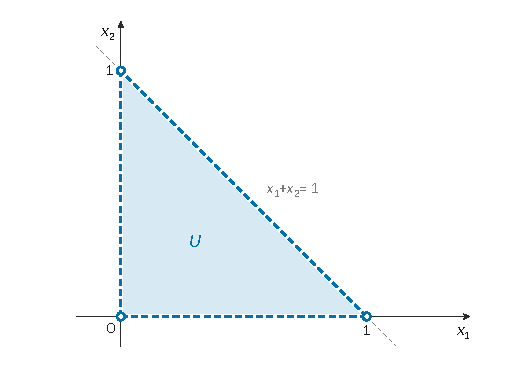
\includegraphics{figures/q5-1-domaine-u.pdf}
\caption*{Figure 1 --- Domaine U pour r = 3 : intérieur du triangle de sommets (0,
0), (1, 0), (0, 1), côtés et sommets exclus}
\end{figure}

\hypertarget{section-9}{%
\subsubsection{5.2.}\label{section-9}}

\emph{Ouvert.} Pour \(1\le k\le r-1\), l'application \(x\mapsto x_k\) est linéaire sur \(\mathbb R^{r-1}\), donc continue. Il en va de même de \(x\mapsto\sum_{j=1}^{r-1}x_j\).

Chaque ensemble \(\{x_k>0\}\) est l'image réciproque de l'ouvert \(]0,+\infty[\) ; l'ensemble \(\{\sum_j x_j<1\}\) est l'image réciproque de l'ouvert \(]-\infty,1[\). Ce sont donc des ouverts.

\(U\) est l'intersection de ces \(r\) ouverts (\(r-1\) conditions de positivité et une condition sur la somme) : intersection finie d'ouverts, \textbf{\(U\) est ouvert}.

\emph{Borné.} Soit \(x\in U\) et \(k\in[\![1,r-1]\!]\). Les autres \(x_j\) étant positifs :
\equationajustee{0<x_k\le\sum_{j=1}^{r-1}x_j<1.}
Donc \(U\subset\,]0,1[^{r-1}\) et \(\|x\|_\infty<1\) : \textbf{\(U\) est borné}.

\hypertarget{section-10}{%
\subsubsection{5.3.}\label{section-10}}

Sous la contrainte, \(x_r=1-\sum_{j=1}^{r-1}x_j\). Pour \((x_1,\dots,x_{r-1})\in U\), on a bien \(x_r\in\,]0,1[\), et \(1-x_r=\sum_{j=1}^{r-1}x_j\).

Ainsi \(U\) décrit exactement les \(r-1\) premières coordonnées des \(r\)-uplets admissibles, et
\equationajustee{\boxed{\begin{aligned}{}&h(x_1,\dots,x_{r-1})\\
&\quad=\sum_{j=1}^{r-1}(1-x_j)^n+\Big(\sum_{j=1}^{r-1}x_j\Big)^n.
\end{aligned}}}
On a bien \(h(x_1,\dots,x_{r-1})=\mathbb E(X)\), et \(h\) ne dépend que des \(r-1\) variables libres.

\hypertarget{section-11}{%
\subsubsection{5.4.}\label{section-11}}

\(h\) est une fonction polynomiale en \((x_1,\dots,x_{r-1})\) : c'est une somme de puissances de fonctions affines.

Une fonction polynomiale est de classe \(\mathcal C^\infty\) sur \(\mathbb R^{r-1}\). Donc \textbf{\(h\) est de classe \(\mathcal C^2\) (et même \(\mathcal C^\infty\)) sur l'ouvert \(U\)}.

\hypertarget{section-12}{%
\subsubsection{5.5.1.}\label{section-12}}

Notons \(s=\sum_{k=1}^{r-1}x_k\), de sorte que \(\frac{\partial s}{\partial x_j}=1\). Alors :
\equationajustee{\boxed{\begin{aligned}
\frac{\partial h}{\partial x_j}(m)&=-n(1-x_j)^{n-1}+n\,s^{\,n-1}\\
&=n\Big[\Big(\sum_{k=1}^{r-1}x_k\Big)^{n-1}-(1-x_j)^{n-1}\Big].
\end{aligned}}}

\hypertarget{section-13}{%
\subsubsection{5.5.2.}\label{section-13}}

Sur \(U\), on a \(s>0\) et \(1-x_j>0\). La fonction \(t\mapsto t^{n-1}\) est strictement croissante sur \(]0,+\infty[\) (car \(n-1\ge1\)), donc injective. Par suite :
\equationajustee{\begin{aligned}
\nabla h(m)=0&\iff\forall j\in[\![1,r-1]\!],\ (1-x_j)^{n-1}=s^{n-1}\\
&\iff\forall j\in[\![1,r-1]\!],\ 1-x_j=s.
\end{aligned}}

Tous les \(x_j\) sont alors égaux à \(c=1-s\). On en tire \(s=(r-1)c\), puis \(1-c=(r-1)c\), d'où \(c=\frac1r\).

Réciproquement, le point \((\frac1r,\dots,\frac1r)\) est dans \(U\) (coordonnées \(>0\), somme \(\frac{r-1}r<1\)) et annule le gradient. L'unique point critique de \(h\) sur \(U\) est
\equationajustee{\boxed{b=\Big(\frac1r,\dots,\frac1r\Big)\in\mathbb R^{r-1}.}}

\hypertarget{section-14}{%
\subsubsection{5.6.1.}\label{section-14}}

Pour \(i,j\in[\![1,r-1]\!]\), en dérivant 5.5.1 :
\equationajustee{\frac{\partial^2h}{\partial x_i\partial x_j}(m)=n(n-1)\,s^{\,n-2}+\delta_{ij}\,n(n-1)(1-x_j)^{n-2}.}

En \(b\), on a \(s=\frac{r-1}r\) et \(1-x_j=\frac{r-1}r\). Posons
\equationajustee{A=n(n-1)\Big(\frac{r-1}r\Big)^{n-2}>0.}
Avec \(J\) la matrice de 3. de taille \(p=r-1\ge2\) :
\equationajustee{\boxed{H_h(b)=A\,(I_{r-1}+J).}}
C'est la matrice de taille \(r-1\) de coefficients diagonaux \(2A\) et non diagonaux \(A\).

\hypertarget{section-15}{%
\subsubsection{5.6.2.}\label{section-15}}

D'après 3.3 (avec \(p=r-1\ge2\)), \(I_{r-1}+J\in\mathcal S^{++}_{r-1}(\mathbb R)\). Comme \(A>0\), \(H_h(b)=A(I_{r-1}+J)\) est symétrique définie positive : pour \(V\ne0\),
\equationajustee{V^TH_h(b)V=A\,V^T(I_{r-1}+J)V>0.}

Récapitulons les hypothèses de la condition suffisante du second ordre :

\begin{itemize}
\tightlist
\item
  \(h\) est de classe \(\mathcal C^2\) sur l'ouvert \(U\) (5.2 et 5.4) ;
\item
  \(b\) est un point critique de \(h\) (5.5.2) ;
\item
  \(H_h(b)\in\mathcal S^{++}_{r-1}(\mathbb R)\).
\end{itemize}

Donc \textbf{\(h\) admet en \(b\) un minimum local strict}. Comme \(h=\mathbb E(X)\) et qu'en \(b\) on a \(x_r=1-\frac{r-1}r=\frac1r\) :
\equationajustee{\boxed{\begin{aligned}{}&\mathbb E(X)\ \text{admet un minimum local}\\
&\text{pour } x_1=\dots=x_r=\tfrac1r.
\end{aligned}}}

\hypertarget{section-16}{%
\subsubsection{5.6.3.}\label{section-16}}

Soit \((x_1,\dots,x_r)\in\,]0,1[^r\) avec \(\sum_j x_j=1\). Posons \(u_j=1-x_j\in\,]0,1[\).

On a \(\sum_{j=1}^r u_j=r-1\). Notons \(\mu\) la moyenne des \(u_j\) :
\equationajustee{\begin{aligned}
\mu&=\frac1r\sum_{j=1}^r u_j\\
&=\frac{r-1}r\in\,]0,1[.
\end{aligned}}

\emph{Inégalité.} L'inégalité de Jensen (question 2) avec les poids \(\frac1r\) donne :
\equationajustee{\begin{aligned}
\mu^n&=\Big(\frac1r\sum_{j=1}^r u_j\Big)^n\\
&\le\frac1r\sum_{j=1}^r u_j^n\\
&=\frac1r\,\mathbb E(X).
\end{aligned}}
Donc \(\mathbb E(X)\ge r\big(\frac{r-1}r\big)^n\). Cette borne est atteinte pour \(x_1=\dots=x_r=\frac1r\), où \(\mathbb E(X)=r\big(1-\frac1r\big)^n\).

\emph{Cas d'égalité.} Pour \(t\in\,]0,1[\), posons
\equationajustee{g(t)=\varphi(t)-\varphi(\mu)-\varphi'(\mu)(t-\mu).}
On a aussi \(g(t)=\int_\mu^t\big(\varphi'(v)-\varphi'(\mu)\big)\,dv\).

Comme \(\varphi'\) est strictement croissante sur \(]0,1[\) (question 1), l'intégrande est du signe de \(v-\mu\). Donc \textbf{\(g(t)>0\) pour \(t\ne\mu\)}, et \(g(\mu)=0\).

En sommant, et puisque \(\sum_{j=1}^r(u_j-\mu)=0\) :
\equationajustee{\begin{aligned}
\sum_{j=1}^r g(u_j)&=\sum_{j=1}^r u_j^n-r\mu^n-\varphi'(\mu)\sum_{j=1}^r(u_j-\mu)\\
&=\mathbb E(X)-r\Big(\frac{r-1}r\Big)^n.
\end{aligned}}

Une somme de termes positifs est nulle si et seulement si chacun l'est. Donc \(\mathbb E(X)=r\big(\frac{r-1}r\big)^n\) si et seulement si \(u_j=\mu\) pour tout \(j\), c'est-à-dire \(x_j=\frac1r\) pour tout \(j\).

Le minimum de \(\mathbb E(X)\) sous la contrainte vaut donc \(r\big(\frac{r-1}r\big)^n\), et
\equationajustee{\boxed{\begin{aligned}{}&\mathbb E(X)\ \text{est minimale}\\
&\text{si, et seulement si, } x_1=\dots=x_r=\tfrac1r.
\end{aligned}}}

\hypertarget{exercice-2}{%
\section{Exercice 2}\label{exercice-2}}

\hypertarget{question-de-cours}{%
\subsection{Question de cours}\label{question-de-cours}}

\hypertarget{section-17}{%
\subsubsection{1.}\label{section-17}}

La série de Riemann \(\sum_{n\ge1}\frac1{n^x}\) \textbf{converge si et seulement si \(x>1\)}. On note alors \(\zeta(x)=\sum_{n=1}^{+\infty}\frac1{n^x}\).

\hypertarget{section-18}{%
\subsubsection{2.}\label{section-18}}

La série entière \(\sum_{n\ge0}t^n\) a pour rayon de convergence \(1\). Son intervalle de convergence est \(]-1,1[\) : elle diverge grossièrement en \(1\) et en \(-1\). Sa somme est donnée par
\equationajustee{\boxed{\begin{aligned}{}&\forall t\in\,]-1,1[,\\
&\sum_{n=0}^{+\infty}t^n=\frac1{1-t}.
\end{aligned}}}

\hypertarget{les-fonctions-e_k}{%
\subsection{\texorpdfstring{Les fonctions \(E_k\)}{Les fonctions E\_k}}\label{les-fonctions-e_k}}

\hypertarget{section-19}{%
\subsubsection{3.}\label{section-19}}

Soit \(x\in\mathbb R\setminus\mathbb Z\). Alors \(x\neq0\), et pour \(n\ge1\), \(x\pm n\neq0\). On a :
\equationajustee{\frac1{x-n}+\frac1{x+n}=\frac{2x}{x^2-n^2}.}

Ce terme change de signe selon \(n\) ; on étudie donc sa valeur absolue :
\equationajustee{\Big|\frac{2x}{x^2-n^2}\Big|\underset{n\to+\infty}{\sim}\frac{2|x|}{n^2}.}
La série de Riemann \(\sum\frac1{n^2}\) converge. Par comparaison de séries à termes positifs, la série \(\sum_{n\ge1}\big(\frac1{x-n}+\frac1{x+n}\big)\) \textbf{converge absolument}, donc converge.

Avec \(\frac1x\) défini, \textbf{\(E_1(x)\) existe pour tout \(x\in\mathbb R\setminus\mathbb Z\)}.

(Les séries \(\sum\frac1{x-n}\) et \(\sum\frac1{x+n}\), prises séparément, divergent : seul le regroupement par paires converge.)

\hypertarget{section-20}{%
\subsubsection{4.1.}\label{section-20}}

Soit \(k\ge2\). Pour \(n\ge1\), \(x\pm n\ne0\), et
\equationajustee{\Big|\frac1{(x\pm n)^k}\Big|=\frac1{|x\pm n|^k}\underset{n\to+\infty}{\sim}\frac1{n^k}.}
Comme \(k>1\), la série \(\sum\frac1{n^k}\) converge. Par comparaison de séries à termes positifs, \textbf{les séries \(\sum_{n\ge1}\frac1{(x-n)^k}\) et \(\sum_{n\ge1}\frac1{(x+n)^k}\) convergent absolument}, donc convergent.

\hypertarget{section-21}{%
\subsubsection{4.2.}\label{section-21}}

\(\frac1{x^k}\) est défini car \(x\neq0\), et les deux séries de 4.1 convergent : \textbf{\(E_k(x)\) existe pour tout \(x\in\mathbb R\setminus\mathbb Z\) et tout \(k\ge2\)}.

Pour tout \(k\ge1\), on pose
\equationajustee{u_{k,n}(x)=\frac1{(x-n)^k}+\frac1{(x+n)^k}.}
Ainsi \(E_k(x)=\frac1{x^k}+\sum_{n=1}^{+\infty}u_{k,n}(x)\). Pour \(k\ge2\), c'est la somme des deux séries convergentes de 4.1.

\hypertarget{section-22}{%
\subsubsection{5.1.}\label{section-22}}

Soit \(k\ge1\) et \(x\in\mathbb R\setminus\mathbb Z\) ; alors \(x+1\in\mathbb R\setminus\mathbb Z\). Pour \(N\ge1\), posons
\equationajustee{\begin{aligned}
S_N(x)&=\frac1{x^k}+\sum_{n=1}^N u_{k,n}(x)\\
&=\sum_{m=-N}^{N}\frac1{(x+m)^k},
\end{aligned}}
de sorte que \(S_N(x)\to E_k(x)\). Par décalage d'indice dans cette somme finie :
\equationajustee{\begin{aligned}
S_N(x+1)&=\sum_{m=-N}^{N}\frac1{(x+1+m)^k}\\
&=\sum_{m=-N+1}^{N+1}\frac1{(x+m)^k}\\
&=S_N(x)-\frac1{(x-N)^k}+\frac1{(x+N+1)^k}.
\end{aligned}}
Les deux derniers termes tendent vers \(0\) quand \(N\to+\infty\). En passant à la limite :
\equationajustee{\boxed{\forall k\ge1,\ \forall x\in\mathbb R\setminus\mathbb Z,\quad E_k(x+1)=E_k(x).}}
\textbf{\(E_k\) est 1-périodique.}

\hypertarget{section-23}{%
\subsubsection{5.2.}\label{section-23}}

\(\mathbb R\setminus\mathbb Z\) est symétrique par rapport à \(0\). Pour \(n\ge1\) :
\equationajustee{\begin{aligned}
u_{k,n}(-x)&=\frac1{(-x-n)^k}+\frac1{(-x+n)^k}\\
&=(-1)^k\Big(\frac1{(x+n)^k}+\frac1{(x-n)^k}\Big)\\
&=(-1)^ku_{k,n}(x).
\end{aligned}}
De plus \(\frac1{(-x)^k}=\frac{(-1)^k}{x^k}\).

On somme la série convergente des \(u_{k,n}\). Cela vaut aussi pour \(k=1\), où l'on ne sépare jamais les deux séries :
\equationajustee{\boxed{E_k(-x)=(-1)^kE_k(x).}}
\textbf{\(E_k\) est paire si \(k\) est pair, impaire si \(k\) est impair.}

\hypertarget{une-relation-de-ruxe9currence}{%
\subsection{6. Une relation de récurrence}\label{une-relation-de-ruxe9currence}}

\hypertarget{section-24}{%
\subsubsection{6.1.}\label{section-24}}

Soit \(k\ge1\) et \(p\in\mathbb Z\). On travaille sur l'intervalle \(I_p=\,]p,p+1[\), car le théorème de dérivation terme à terme porte sur un intervalle.

\begin{itemize}
\tightlist
\item
  Chaque \(u_{k,n}\) est de classe \(\mathcal C^1\) sur \(I_p\), de dérivée \(u_{k,n}'=-k\,u_{k+1,n}\).
\item
  La série \(\sum_n u_{k,n}\) converge simplement sur \(I_p\) (questions 3 et 4).
\item
  Soit \([\alpha,\beta]\subset I_p\) et \(A=\max(|\alpha|,|\beta|)\). Pour \(n\ge2A\) et \(x\in[\alpha,\beta]\), on a \(|x\pm n|\ge n-|x|\ge\frac n2\), donc :
\end{itemize}

\equationajustee{\begin{aligned}
\sup_{[\alpha,\beta]}|u_{k,n}'|&\le 2k\Big(\frac2n\Big)^{k+1}\\
&=\frac{2^{k+2}k}{n^{k+1}}.
\end{aligned}}

C'est le terme général d'une série convergente, puisque \(k+1\ge2\). La série \(\sum u_{k,n}'\) converge donc normalement, donc uniformément, sur tout segment de \(I_p\).

Par le théorème de dérivation terme à terme des séries de fonctions, \(x\mapsto\sum_{n\ge1}u_{k,n}(x)\) est de classe \(\mathcal C^1\) sur \(I_p\), de dérivée \(\sum_{n\ge1}u_{k,n}'\).

Avec \(\big(\frac1{x^k}\big)'=-\frac k{x^{k+1}}\), on obtient sur \(I_p\), donc sur \(\mathbb R\setminus\mathbb Z=\bigcup_p I_p\) :
\equationajustee{\begin{aligned}
E_k'(x)&=-\frac k{x^{k+1}}-k\sum_{n=1}^{+\infty}u_{k+1,n}(x)\\
&=-k\,E_{k+1}(x).
\end{aligned}}
\equationajustee{\boxed{\forall x\in\mathbb R\setminus\mathbb Z,\quad E_k'(x)=-k\,E_{k+1}(x).}}

\hypertarget{section-25}{%
\subsubsection{6.2.}\label{section-25}}

\emph{Régularité.} Pour \(q\in\mathbb N\), notons \(\mathcal P(q)\) : « pour tout \(k\ge1\), \(E_k\) est de classe \(\mathcal C^q\) sur \(\mathbb R\setminus\mathbb Z\) ».

\begin{itemize}
\item
  \(\mathcal P(0)\) est vraie : chaque \(E_k\) est dérivable (6.1), donc continue.
\item
  Supposons \(\mathcal P(q)\) et fixons \(k\ge1\). D'après 6.1, \(E_k\) est dérivable et \(E_k'=-kE_{k+1}\).

  Par \(\mathcal P(q)\), \(E_{k+1}\) est de classe \(\mathcal C^q\), donc \(E_k'\) aussi.
\item
  Ainsi \(E_k\) est de classe \(\mathcal C^{q+1}\) pour tout \(k\ge1\) : \(\mathcal P(q+1)\) est vraie.
\end{itemize}

Ainsi \textbf{chaque \(E_k\) est de classe \(\mathcal C^\infty\) sur \(\mathbb R\setminus\mathbb Z\)}.

\emph{Formule.} Par récurrence sur \(k\ge1\). Pour \(k=1\), la formule s'écrit \(E_1=\frac{(-1)^0}{0!}E_1^{(0)}\) : elle est vraie.

Supposons \(E_k=\frac{(-1)^{k-1}}{(k-1)!}E_1^{(k-1)}\). Par 6.1 :
\equationajustee{\begin{aligned}
E_{k+1}&=-\frac1kE_k'\\
&=-\frac1k\cdot\frac{(-1)^{k-1}}{(k-1)!}E_1^{(k)}\\
&=\frac{(-1)^k}{k!}E_1^{(k)}.
\end{aligned}}
\equationajustee{\boxed{\forall k\ge1,\quad E_k=\frac{(-1)^{k-1}}{(k-1)!}E_1^{(k-1)}.}}

\hypertarget{section-26}{%
\subsubsection{7.}\label{section-26}}

Soit \(x\in\,]-1,1[\) et \(n\ge1\). Alors \(\big|\frac xn\big|\le|x|<1\).

Par la question 2, la série géométrique \(\sum_k\big(\frac xn\big)^k\) converge, de somme \(\frac1{1-x/n}=\frac n{n-x}\) (avec \(n-x>0\)).

Par suite, \(\sum_{k\ge0}\frac{x^k}{n^{k+1}}=\frac1n\sum_{k\ge0}\big(\frac xn\big)^k\) converge, et
\equationajustee{\boxed{\sum_{k=0}^{+\infty}\frac{x^k}{n^{k+1}}=\frac1{n-x}.}}

\hypertarget{section-27}{%
\subsubsection{8.}\label{section-27}}

Soit \(x\in\,]-1,1[\) et \(n\ge1\). La question 7, appliquée à \(x\) et à \(-x\), donne
\equationajustee{\begin{aligned}
\frac1{n-x}-\frac1{n+x}&=\sum_{k=0}^{+\infty}\frac{x^k-(-x)^k}{n^{k+1}}\\
&=\sum_{k=0}^{+\infty}\frac{(1-(-1)^k)\,x^k}{n^{k+1}}.
\end{aligned}}

Les termes d'indice pair sont nuls. Ceux d'indice impair \(k=2s-1\) valent \(\frac{2x^{2s-1}}{n^{2s}}\). Supprimer des termes nuls ne change ni la convergence ni la somme :
\equationajustee{\frac1{n-x}-\frac1{n+x}=\sum_{s=1}^{+\infty}\frac2{n^{2s}}x^{2s-1}.}

Le membre de gauche vaut \(\frac{2x}{n^2-x^2}=O\big(\frac1{n^2}\big)\) : c'est le terme général d'une série convergente. En sommant sur \(n\ge1\) l'égalité précédente, sans aucune interversion :
\equationajustee{\boxed{\begin{aligned}{}&\sum_{n=1}^{+\infty}\Big(\frac1{n-x}-\frac1{n+x}\Big)\\
&\qquad=\sum_{n=1}^{+\infty}\sum_{s=1}^{+\infty}\frac2{n^{2s}}x^{2s-1}.
\end{aligned}}}

\hypertarget{section-28}{%
\subsubsection{9.}\label{section-28}}

Soit \(x\in\,]-1,1[\), \(x\ne0\). Comme \(\frac1{x-n}+\frac1{x+n}=-\big(\frac1{n-x}-\frac1{n+x}\big)\), la question 8 donne
\equationajustee{\begin{aligned}
E_1(x)&=\frac1x-\sum_{n=1}^{+\infty}\sum_{s=1}^{+\infty}a_{n,s},\\
a_{n,s}&=\frac{2x^{2s-1}}{n^{2s}}.
\end{aligned}}

\textbf{Théorème utilisé (Fubini pour les séries doubles).} Soit \((a_{n,s})_{(n,s)\in\mathbb N^*\times\mathbb N^*}\) une famille de nombres complexes. On suppose :

\begin{itemize}
\tightlist
\item
  pour tout \(n\), la série \(\sum_s|a_{n,s}|\) converge ;
\item
  la série \(\sum_n\Big(\sum_{s=1}^{+\infty}|a_{n,s}|\Big)\) converge.
\end{itemize}

Alors la famille est sommable. Pour tout \(s\), la série \(\sum_n a_{n,s}\) converge ; pour tout \(n\), la série \(\sum_s a_{n,s}\) converge ; et
\equationajustee{\begin{aligned}{}&\sum_{n=1}^{+\infty}\sum_{s=1}^{+\infty}a_{n,s}\\
&\qquad=\sum_{s=1}^{+\infty}\sum_{n=1}^{+\infty}a_{n,s}.
\end{aligned}}

\textbf{Vérification des hypothèses.} Fixons \(n\ge1\). La série \(\sum_s|a_{n,s}|=\sum_{s\ge1}\frac{2|x|}{n^2}\Big(\frac{x^2}{n^2}\Big)^{s-1}\) est géométrique de raison \(\frac{x^2}{n^2}\in[0,1[\). Elle converge, de somme
\equationajustee{\begin{aligned}
\sum_{s=1}^{+\infty}|a_{n,s}|&=\frac{2|x|}{n^2}\cdot\frac1{1-x^2/n^2}\\
&=\frac{2|x|}{n^2-x^2}\\
&\le\frac{2|x|}{n^2(1-x^2)},
\end{aligned}}
la dernière inégalité venant de \(n^2-x^2\ge n^2-n^2x^2\).

La série \(\sum_n\frac{2|x|}{n^2(1-x^2)}\) converge, donc \(\sum_n\sum_s|a_{n,s}|\) converge. Les hypothèses sont vérifiées.

\textbf{Conclusion.} Pour \(s\ge1\), comme \(2s>1\) :
\equationajustee{\sum_{n\ge1}a_{n,s}=2x^{2s-1}\sum_{n\ge1}\frac1{n^{2s}}=2\zeta(2s)x^{2s-1}.}
D'où la convergence de \(\sum_s\zeta(2s)x^{2s-1}\), et
\equationajustee{\boxed{E_1(x)=\frac1x-2\sum_{s=1}^{+\infty}\zeta(2s)\,x^{2s-1}.}}

\hypertarget{section-29}{%
\subsubsection{10.}\label{section-29}}

Posons \(g(x)=\sum_{s\ge1}\zeta(2s)x^{2s-1}\). D'après 9, cette série entière converge en tout point de \(]-1,1[\), donc son rayon de convergence vérifie \(R\ge1\). (Il vaut d'ailleurs \(1\) : \(\zeta(2s)\ge1\), et la série diverge grossièrement en \(x=1\).)

Sa somme \(g\) est donc de classe \(\mathcal C^\infty\) sur \(]-1,1[\) et s'y dérive terme à terme à tout ordre. Pour \(q\in\mathbb N\) :
\equationajustee{\begin{aligned}
g^{(q)}(x)&=\sum_{s\ge1,\ 2s-1\ge q}\zeta(2s)\frac{(2s-1)!}{(2s-1-q)!}x^{2s-1-q}\\
&=q!\sum_{s=1}^{+\infty}\binom{2s-1}{q}\zeta(2s)\,x^{2s-1-q}.
\end{aligned}}
Les termes tels que \(q>2s-1\) sont des dérivées \(q\)-ièmes de monômes de degré \(<q\), donc nuls : ils correspondent exactement à la convention \(\binom{2s-1}q=0\).

Sur chacun des intervalles ouverts \(]-1,0[\) et \(]0,1[\), on a \(E_1(x)=\frac1x-2g(x)\) (question 9). Soit \(k\ge1\). On dérive \(k-1\) fois, avec \(\big(\frac1x\big)^{(k-1)}=\frac{(-1)^{k-1}(k-1)!}{x^k}\) :
\equationajustee{E_1^{(k-1)}(x)=\frac{(-1)^{k-1}(k-1)!}{x^k}-2(k-1)!\sum_{s=1}^{+\infty}\binom{2s-1}{k-1}\zeta(2s)\,x^{2s-k}.}

Par 6.2, \(E_k=\frac{(-1)^{k-1}}{(k-1)!}E_1^{(k-1)}\). Avec \(-(-1)^{k-1}=(-1)^k\), on obtient, pour tout \(k\in\mathbb N^*\) et tout \(x\in\,]-1,1[\setminus\{0\}\) :
\equationajustee{\boxed{E_k(x)=\frac1{x^k}+2(-1)^k\sum_{s=1}^{+\infty}\binom{2s-1}{k-1}\zeta(2s)\,x^{2s-k}.}}

\hypertarget{exercice-3}{%
\section{Exercice 3}\label{exercice-3}}

Notations : \(\sigma=\sum_{j=1}^{n-1}a_j^2\) ; \((e_1,\dots,e_n)\) est la base canonique de \(\mathbb K^n\) ; pour \(\lambda\in\mathbb K\), \(F_\lambda=\ker(M-\lambda I_n)\).

\hypertarget{cas-mathbb-kmathbb-r}{%
\subsection{\texorpdfstring{1. Cas \(\mathbb K=\mathbb R\)}{1. Cas \textbackslash mathbb K=\textbackslash mathbb R}}\label{cas-mathbb-kmathbb-r}}

\hypertarget{section-30}{%
\subsubsection{1.1.}\label{section-30}}

Pour \(i<n\), \(M_{i,n}=a_i=M_{n,i}\). Les autres coefficients hors de la dernière ligne et de la dernière colonne sont nuls. Donc \(M^T=M\).

Les coefficients \(a_j\) sont \textbf{réels} : \(M\) est une matrice \textbf{symétrique réelle}. D'après le théorème spectral, elle est \textbf{diagonalisable} (dans une base orthonormée).

\hypertarget{section-31}{%
\subsubsection{1.2.}\label{section-31}}

Pour \(j\le n-1\), la colonne \(C_j\) vaut \(a_j e_n\). La dernière colonne est \(C_n=(a_1,\dots,a_n)^T\). Donc
\equationajustee{\mathrm{Im}\,M=\mathrm{Vect}(C_1,\dots,C_n)\subset\mathrm{Vect}(e_n,C_n),}
et \(\mathrm{rg}\,M\le2\).

Par ailleurs, \(C_1=a_1e_n\neq0\). La colonne \(C_n\), de première coordonnée \(a_1\neq0\), n'est pas colinéaire à \(e_n\). La famille \((C_1,C_n)\) est donc libre, et
\equationajustee{\boxed{\mathrm{rg}\,M=2.}}

\hypertarget{section-32}{%
\subsubsection{1.3.}\label{section-32}}

Par le théorème du rang, \(\dim\ker M=n-\mathrm{rg}\,M=n-2\ge1\) (car \(n\ge3\)). Le noyau n'est pas réduit à \(\{0\}\) : \textbf{\(0\) est valeur propre}, et son sous-espace propre est de dimension \(n-2\).

L'ordre de multiplicité est la multiplicité de \(0\) comme racine de \(\chi_M\). En général, la dimension du sous-espace propre est seulement inférieure ou égale à cette multiplicité. Ici, \(M\) est diagonalisable (1.1) : il y a égalité. Donc \textbf{\(0\) est valeur propre de multiplicité \(n-2\)}.

\hypertarget{section-33}{%
\subsubsection{1.4.}\label{section-33}}

\(M\) est diagonalisable, donc \(\chi_M\) est scindé sur \(\mathbb R\), de degré \(n\). La somme des multiplicités des valeurs propres vaut donc \(n\).

Comme \(0\) a pour multiplicité exactement \(n-2\), les autres valeurs propres sont non nulles, de multiplicité totale \(2\). Ainsi \(M\) possède \textbf{deux valeurs propres non nulles \(\lambda_1,\lambda_2\)} (comptées avec multiplicité), et
\equationajustee{\chi_M(X)=X^{n-2}(X-\lambda_1)(X-\lambda_2).}
(On verra en 1.6 qu'elles sont en fait distinctes.)

\hypertarget{section-34}{%
\subsubsection{1.5.}\label{section-34}}

Le système \(MX=0\) s'écrit \(a_ix_n=0\) pour \(1\le i\le n-1\), et \(\sum_{j=1}^{n-1}a_jx_j+a_nx_n=0\).

Comme \(a_1\ne0\), la première équation donne \(x_n=0\). Il reste
\equationajustee{\begin{aligned}
\ker M=\Big\{X\in\mathbb R^n:\ &x_n=0\\
\text{et }\ &\sum_{j=1}^{n-1}a_jx_j=0\Big\}.
\end{aligned}}

Pour \(2\le k\le n-1\), posons \(v_k=a_ke_1-a_1e_k\). Ce vecteur est dans \(\ker M\), car \(a_1a_k-a_ka_1=0\).

Ces vecteurs sont libres : la coordonnée d'indice \(k\) de \(v_k\) vaut \(-a_1\ne0\), et celle des autres \(v_\ell\) est nulle. Ils sont au nombre de \(n-2=\dim\ker M\). Donc
\equationajustee{\boxed{\begin{aligned}
\ker M&=\mathrm{Vect}(v_2,\dots,v_{n-1}),\\
v_k&=(a_k,0,\dots,0,\underbrace{-a_1}_{k},0,\dots,0)^T.
\end{aligned}}}

\hypertarget{section-35}{%
\subsubsection{1.6.}\label{section-35}}

Soit \(\lambda\ne0\) et \(X\ne0\) tel que \(MX=\lambda X\).

Les \(n-1\) premières lignes donnent \(a_ix_n=\lambda x_i\), soit \(x_i=\frac{a_i}\lambda x_n\) pour \(i\le n-1\).

Si \(x_n=0\), tous les \(x_i\) sont nuls et \(X=0\) : c'est exclu. Donc \(x_n\neq0\).

La dernière ligne donne
\equationajustee{\sum_{j=1}^{n-1}a_j\frac{a_j}\lambda x_n+a_nx_n=\lambda x_n.}
En divisant par \(x_n\) et en multipliant par \(\lambda\) :
\equationajustee{\boxed{\lambda^2-\lambda a_n-\sum_{j=1}^{n-1}a_j^2=0.}}

Appliqué à \(\lambda=\lambda_1\) et à \(\lambda=\lambda_2\) (valeurs propres non nulles), ce calcul montre que \textbf{\(\lambda_1\) et \(\lambda_2\) sont solutions de cette équation}.

Son discriminant vaut \(\Delta=a_n^2+4\sigma\ge4a_1^2>0\), et le produit des racines vaut \(-\sigma<0\). Les racines sont donc réelles, \textbf{distinctes et de signes opposés} :
\equationajustee{\lambda_{1}=\frac{a_n-\sqrt{a_n^2+4\sigma}}2<0<\lambda_{2}=\frac{a_n+\sqrt{a_n^2+4\sigma}}2.}

\(M\) possède deux valeurs propres non nulles comptées avec multiplicité, toutes racines de cette équation à deux racines simples. Ce sont donc exactement \(\lambda_1\) et \(\lambda_2\), chacune simple.

\hypertarget{section-36}{%
\subsubsection{1.7.}\label{section-36}}

Soit \(\lambda\in\{\lambda_1,\lambda_2\}\). D'après 1.6, tout vecteur propre s'écrit \(\frac{x_n}{\lambda}(a_1,\dots,a_{n-1},\lambda)^T\). L'espace propre est donc inclus dans \(\mathrm{Vect}(w_\lambda)\), avec \(w_\lambda=(a_1,\dots,a_{n-1},\lambda)^T\).

Réciproquement, pour \(i<n\), \((Mw_\lambda)_i=a_i\lambda=\lambda(w_\lambda)_i\). Et, puisque \(\lambda^2-a_n\lambda-\sigma=0\) :
\equationajustee{\begin{aligned}
(Mw_\lambda)_n&=\sigma+a_n\lambda\\
&=\lambda^2\\
&=\lambda(w_\lambda)_n.
\end{aligned}}
Donc
\equationajustee{\boxed{\begin{aligned}
F_{\lambda_1}&=\mathrm{Vect}\big((a_1,\dots,a_{n-1},\lambda_1)^T\big),\\
F_{\lambda_2}&=\mathrm{Vect}\big((a_1,\dots,a_{n-1},\lambda_2)^T\big).
\end{aligned}}}

\hypertarget{section-37}{%
\subsubsection{1.8.}\label{section-37}}

Les sous-espaces propres \(\ker M\), \(F_{\lambda_1}\) et \(F_{\lambda_2}\) sont en somme directe, car les valeurs propres \(0,\lambda_1,\lambda_2\) sont distinctes. Leurs dimensions totalisent \((n-2)+1+1=n\). La concaténation de leurs bases est donc une base de \(\mathbb R^n\).

Soit \(P\) la matrice de colonnes \(v_2,\dots,v_{n-1},w_{\lambda_1},w_{\lambda_2}\) :
\equationajustee{P=\begin{pmatrix}
a_2&a_3&\cdots&a_{n-1}&a_1&a_1\\
-a_1&0&\cdots&0&a_2&a_2\\
0&-a_1&\cdots&0&a_3&a_3\\
\vdots&&\ddots&\vdots&\vdots&\vdots\\
0&0&\cdots&-a_1&a_{n-1}&a_{n-1}\\
0&0&\cdots&0&\lambda_1&\lambda_2
\end{pmatrix}.}
\(P\) est inversible, et
\equationajustee{\boxed{P^{-1}MP=\mathrm{diag}\Big(\underbrace{0,\dots,0}_{n-2},\ \frac{a_n-\sqrt{a_n^2+4\sigma}}2,\ \frac{a_n+\sqrt{a_n^2+4\sigma}}2\Big).}}

\hypertarget{uxe9tude-du-cas-mathbb-kmathbb-c}{%
\subsection{\texorpdfstring{2. Étude du cas \(\mathbb K=\mathbb C\)}{2. Étude du cas \textbackslash mathbb K=\textbackslash mathbb C}}\label{uxe9tude-du-cas-mathbb-kmathbb-c}}

\hypertarget{section-38}{%
\subsubsection{2.1.}\label{section-38}}

\emph{Polynôme caractéristique.} Soit \(X\in\mathbb C^*\). Dans \(XI_n-M\), la colonne \(j\le n-1\) vaut \(Xe_j-a_je_n\). La dernière colonne vaut \(-\sum_{j<n}a_je_j+(X-a_n)e_n\).

L'opération \(C_n\leftarrow C_n+\sum_{j=1}^{n-1}\frac{a_j}XC_j\) ne change pas le déterminant. Elle remplace la dernière colonne par \(\big(X-a_n-\frac\sigma X\big)e_n\).

La matrice obtenue est triangulaire inférieure, de diagonale \((X,\dots,X,X-a_n-\frac\sigma X)\). D'où, pour \(X\neq0\) :
\equationajustee{\begin{aligned}
\chi_M(X)&=X^{n-1}\Big(X-a_n-\frac\sigma X\Big)\\
&=X^{n-2}\big(X^2-a_nX-\sigma\big).
\end{aligned}}
Deux polynômes égaux en une infinité de points sont égaux. Avec \(Q=X^2-a_nX-\sigma\) :
\equationajustee{\boxed{\chi_M=X^{n-2}Q.}}

\emph{Sous-espaces propres.} Les calculs de 1.2, 1.5 et 1.6 n'utilisent que \(a_1\ne0\) et restent valables sur \(\mathbb C\). Ainsi \(\dim\ker M=n-2\). Pour toute valeur propre \(\lambda\ne0\), \(\dim F_\lambda=1\) (engendré par \((a_1,\dots,a_{n-1},\lambda)^T\)).

\(\chi_M\) est scindé sur \(\mathbb C\). \(M\) est diagonalisable si et seulement si, pour chaque valeur propre, la dimension du sous-espace propre est égale à la multiplicité.

\begin{itemize}
\item
  \textbf{Si \(\sigma=0\)} : \(Q=X(X-a_n)\). Donc \(0\) est racine de \(\chi_M\) de multiplicité au moins \(n-1\).

  Or \(\dim\ker M=n-2\) : \(M\) n'est pas diagonalisable.
\item
  \textbf{Si \(\sigma\ne0\) et \(a_n^2+4\sigma=0\)} : \(Q\) a une racine double \(\mu=\frac{a_n}2\). Elle est non nulle, car \(Q(0)=-\sigma\ne0\).

  Ainsi \(\mu\) est valeur propre de multiplicité \(2\), mais \(\dim F_\mu=1\) : \(M\) n'est pas diagonalisable.
\item
  \textbf{Si \(\sigma\ne0\) et \(a_n^2+4\sigma\ne0\)} : \(Q\) a deux racines distinctes \(\mu_1\neq\mu_2\), non nulles car \(Q(0)\neq0\).

  Alors \(0\) est de multiplicité exactement \(n-2\), égale à \(\dim\ker M\).

  Les \(\mu_i\) sont simples, et \(\dim F_{\mu_i}=1\). Les dimensions totalisent \(n\) : \(M\) est diagonalisable.
\end{itemize}

Les trois cas étant exhaustifs, \(M\) n'est pas diagonalisable si et seulement si
\equationajustee{\boxed{\begin{aligned}{}&\sum_{j=1}^{n-1}a_j^2=0\\
\text{ou}\quad&a_n^2+4\sum_{j=1}^{n-1}a_j^2=0.
\end{aligned}}}

\hypertarget{section-39}{%
\subsubsection{2.2.}\label{section-39}}

Pour \(n=3\), prenons \(a_1=1\), \(a_2=i\), \(a_3=0\). On a bien \(a_1\ne0\), et \(a_1^2+a_2^2=0\) :
\equationajustee{\boxed{M=\begin{pmatrix}0&0&1\\0&0&i\\1&i&0\end{pmatrix}}}
D'après 2.1, elle n'est pas diagonalisable.

Directement : \(\chi_M=X^3\), donc \(0\) est la seule valeur propre. Si \(M\) était diagonalisable, elle serait semblable à la matrice nulle, donc nulle, ce qui n'est pas le cas. On vérifie d'ailleurs que \(M^3=0\) et que \(M^2\ne0\) :
\equationajustee{M^2=\begin{pmatrix}1&i&0\\i&-1&0\\0&0&0\end{pmatrix}.}

Autre exemple, relevant de la seconde condition : \(a_1=1\), \(a_2=0\), \(a_3=2i\). Alors \(\sigma=1\) et \(a_3^2+4\sigma=0\) ; la valeur propre double \(i\) a un espace propre de dimension 1.

\end{document}
